%\chapterauthor{Author Name}{Author Affiliation}
%\chapterauthor{Second Author}{Second Author Affiliation}
\chapter{File Management} \label{ch:fm}

File management is a big portion of OS. In Linux, each device (such as a printer) is treated and managed as a file, and Linux uses a tree hierarchy to manage devices and files. This chapter introduces the filesystem hierarchy and commonly used file management commands.

\section{Filesystem Hierarchy Standard} \label{ch:fm:sec:hierarchy}

The root directory is denoted by a single forward slash ``\verb|/|''. All sub directories or files can be located by its full path, which looks like the following
\begin{lstlisting}
/<directory>/<subdirectory>/.../<directory-name>
/<directory>/<subdirectory>/.../<file-name>
\end{lstlisting}
where the first \verb|/| in each row represents the root directory, and sequential \verb|/| represents entering a subdirectory.

Upon Linux installation, a file hierarchy is created. A user can create new files under this hierarchy framework, but should not change the framework itself. The hierarchy is given in Fig. \ref{ch:fm:fig:hierarchy}. Notice that different Linux distributions may differ slightly on how the architecture looks like. The ``\verb|/|'' in the figure, as introduced, stands for the root directory, and ``\verb|root|'' in the figure is a subdirectory under \verb|/| whose directory name is ``root'' and it is used store root user related documents. They are two different directories.

\begin{figure}[htbp]
	\centering
	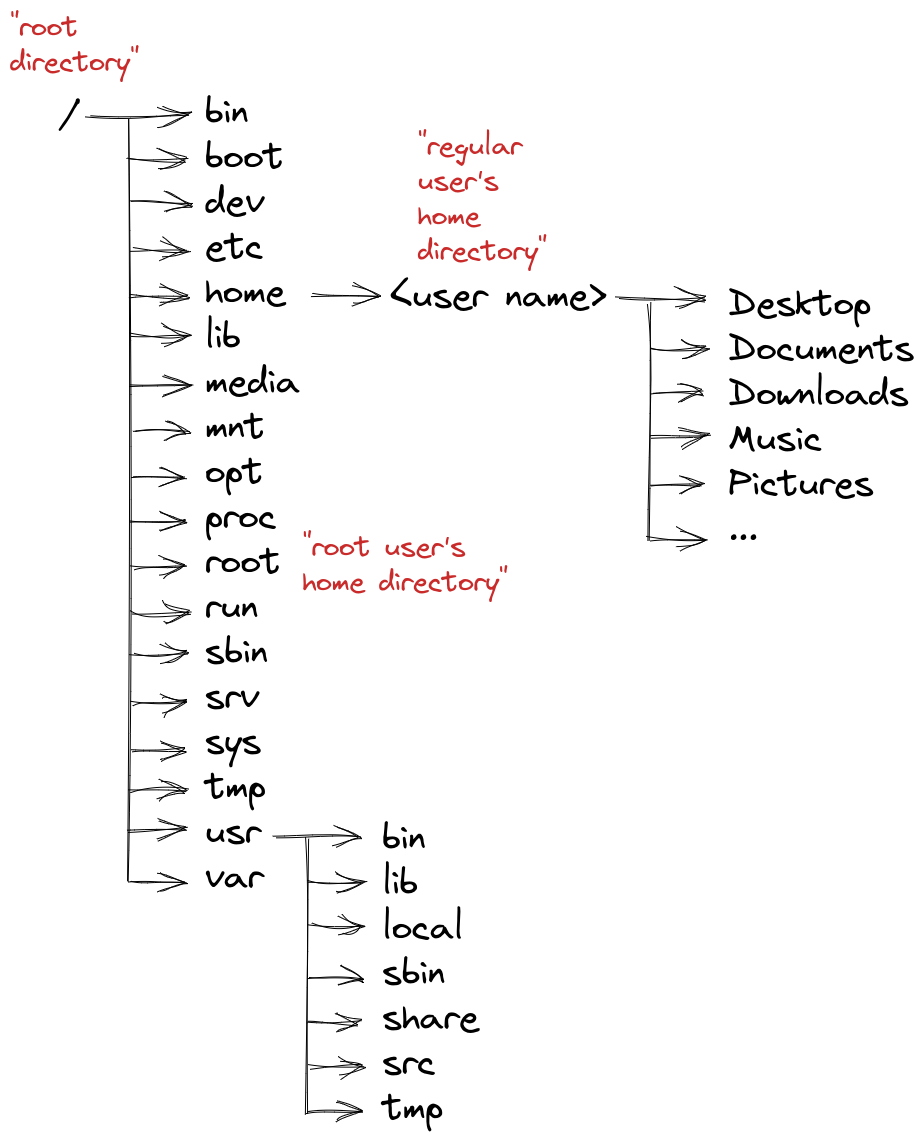
\includegraphics[width=250pt]{chapters/part-1/figures/linux_file_hierarchy.png}
	\caption{An example of Linux file system hierarchy.} \label{ch:fm:fig:hierarchy}
\end{figure}

A regular user's home directory is often located at \verb|/home/<user name>|. When logging in as a regular user, his home directory is stored in the HOME environment and can be retrieved by \verb|$HOME|. A shortcut to \verb|$HOME| is given by the tilde \verb|~| for convenience. Hence, for example \verb|ls ~| lists down the files and directories under his home directory.

As can be seen from Fig. \ref{ch:fm:fig:hierarchy}, the hierarchy contains quite a few pre-determined subdirectories, each serving a different purpose. For the ease of illustration, these subdirectories are roughly categorized by functionalities and accessibility shown in Fig. \ref{ch:fm:fig:directorycate}.

\begin{figure}[htbp]
	\centering
	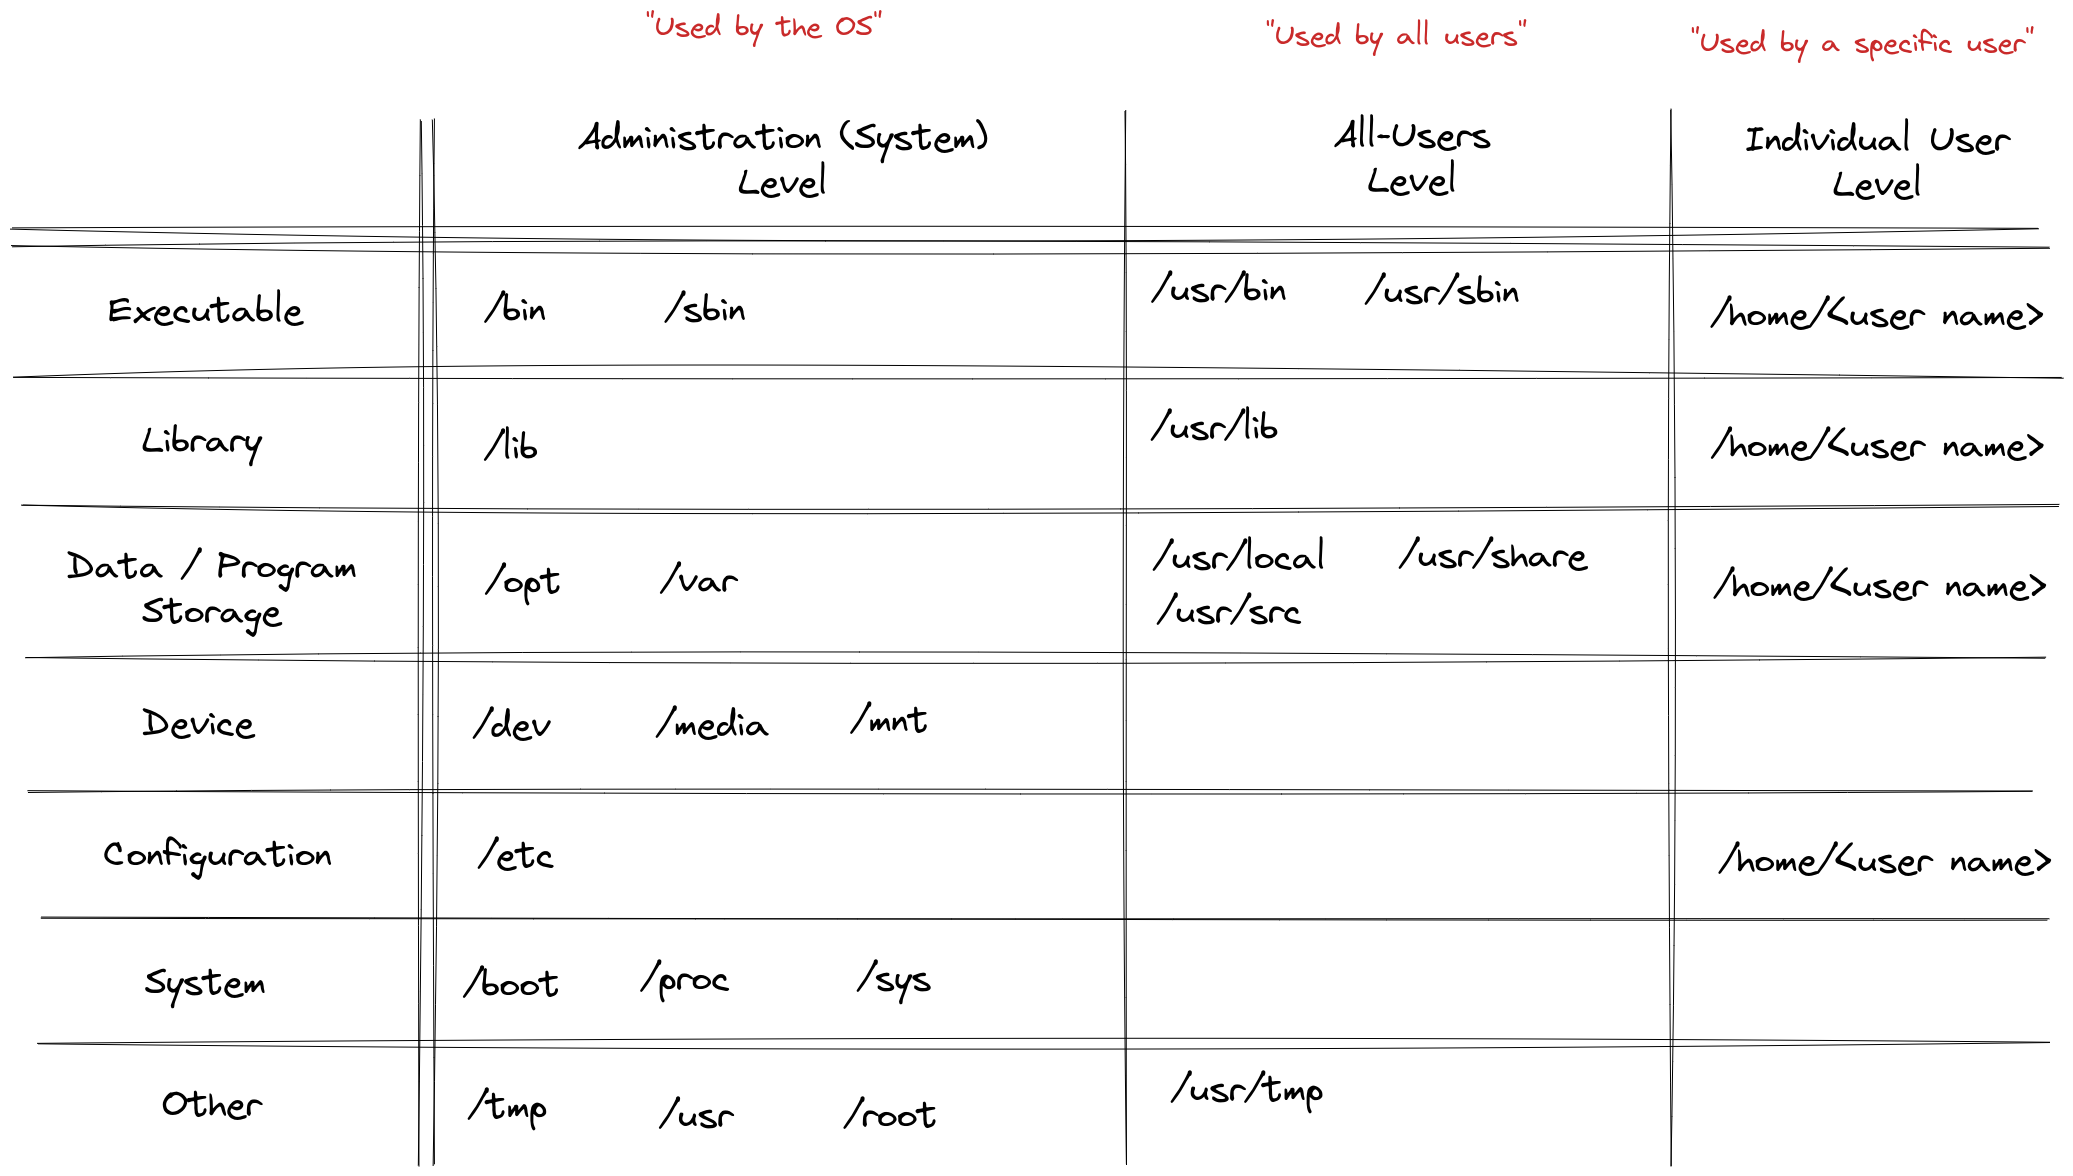
\includegraphics[width=350pt]{chapters/part-1/figures/linux_directory_cate.png}
	\caption{A rough categorization of commonly used directories in Linux file hierarchy standard.} \label{ch:fm:fig:directorycate}
\end{figure}

A brief introduction to the directories are summarized in Table \ref{ch:fm:tab:hierarchyintro}.

\begin{table}
  \centering \caption{Introduction to commonly used directories in Linux file hierarchy standard.}\label{ch:fm:tab:hierarchyintro}
  \begin{tabularx}{\textwidth}{lX}
    \hline
    Directory & Description \\ \hline
    \verb|/bin|, \verb|/sbin| & Executables used by the OS, the administrator, and the regular users. \\ 
    \verb|/lib| & Libraries to support \verb|/bin| and \verb|/sbin|. \\ 
    \verb|/usr/bin|, \verb|/usr/sbin| & Executables used by the administrator and the regular users. \\ 
    \verb|/usr/lib| & Libraries to support \verb|/usr/bin| and \verb|/usr/sbin|. \\ 
    \verb|/opt| & Application software installed by OS and administrator for all users. \\ 
    \verb|/var| & Directories of data used by applications. \\ 
    \verb|/usr/local| & Application software installed by administrator for all users. \\ 
    \verb|/usr/share| & Architecture-independent sharable text files for applications. \\ 
    \verb|/usr/src| & Source files or packages managed by software manager. \\ 
    \verb|/dev| & Files representation of devices, such as CPU, RAM, hard disks. \\ 
    \verb|/media| & System mounts of removable media. \\ 
    \verb|/mnt| & Manual mounts of devices. \\ 
    \verb|/etc| & Configuration files for OS, users, and applications. \\ 
    \verb|/boot| & Linux bootable kernel and initial setups. \\ 
    \verb|/proc| & System resources information. \\ 
    \verb|/sys| & Linux kernel information, including a mirror of the kernel data structure. \\ 
    \verb|/tmp|, \verb|usr/tmp| & Temporary files. \\ 
    \verb|/root| & Root user's home directory. \\ 
    \verb|/home/<user name>| & A regular user's home directory, containing executables, configurations and files specifically belong to this user. \\
    \hline
  \end{tabularx}
\end{table}

Linux file hierarchy standard differs from MS-DOS and Windows in several ways. Firstly, Linux stores all files (regardless of their physical location) under the root directory, while Windows uses drive letters such as \verb|C:\|, \verb|D:\| to distinguish different hard drives. Secondly, Linux uses slash (\verb|/|) to separate directory names, e.g. \verb|/home/username| while Windows uses back slash (\verb|\|), e.g. \verb|C:\Users\username|. Lastly, Linux uses ``magic numbers'' to indicate file types, while Windows often uses suffixes to tell file types. 

Magic numbers of a file refer to the first few bytes of a file that are unique to a particular file type, for example, PNG file is hex \verb|89 50 4e 47|. Linux compare the magic numbers of a file with an internal database to decide the file types and features. Distinguishing file types using magic numbers can be more reliable than using suffixes, though a bit less intuitive.

\section{Commonly Used File Exploring Commands} \label{ch:fm:sec:filemanagement}

Some of the most widely used file exploring and managing commands are summarized in Table \ref{ch:fm:tab:commonfilecommands}. Notice that \verb|chmod| and \verb|chown| are administration related commands that change the accessibility of a directory or a file, and will be introduced in a later sections together with the Linux permission system. The rest commands are categorized and introduced in the following subsections.

\begin{table}
  \centering \caption{Commonly used commands to navigate in the Linux file system.}\label{ch:fm:tab:commonfilecommands}
  \begin{tabularx}{\textwidth}{lX}
    \hline
    Command & Description \\ \hline
    \verb|pwd| & Print working directory. \\ 
    \verb|ls| & List the subdirectories and files (and their detail information) in a given directory. \\ 
    \verb|touch| & Create an empty file. \\ 
    \verb|mkdir| & Create an empty subdirectory. \\ 
    \verb|mv| & Move (cut-and-paste) a directory or a file; change name of a directory or a file. \\ 
    \verb|cp| & Copy-and-paste a directory or a file. \\ 
    \verb|rm|, \verb|rmdir| & Remove a directory or a file (not to Trash, but just gone). \\ 
    \verb|chmod| & Change permission. \\ 
    \verb|chown| & Change ownership. \\
    \hline
  \end{tabularx}
\end{table}

\subsection{Print Working Directory}

As given in Table \ref{ch:sb:tab:shellenvironmentvars}, \verb|$PWD| is the environmental variables to store the current working directory of the shell. Therefore, to print the current working directory in the console, use command 
\begin{lstlisting}
$ echo $PWD
\end{lstlisting}
Alternatively, use \verb|pwd| as follows which has the same effect.
\begin{lstlisting}
$ pwd
\end{lstlisting}

\subsection{List Information about Files and Directories}

As one of the most frequently used commands, \verb|ls| lists down information about the files and subdirectories in the selected directory, and by default sort the entries alphabetically. The syntax is given below.
\begin{lstlisting}
$ ls [<option>] [<path>]
\end{lstlisting}

An example is given in Fig. \ref{ch:fm:fig:lscommandexample}. As shown in the example, command \verb|ls| alone shows only the name of files and subdirectories excluding hidden items and details of each item. With the additional arguments in the option field, the returns can be customized with more details displayed. For example in Fig. \ref{ch:fm:fig:lscommandexample}, the \verb|-l| argument displays the information in long listing form, which includes the owner and access control list information. More details about files and directories access control list are given in later part of this section.

\begin{figure}[htbp]
	\centering
	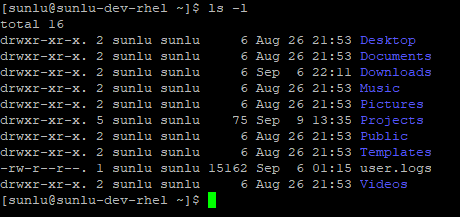
\includegraphics[width=350pt]{chapters/part-1/figures/ls_command_example.png}
	\caption{List down information of files and subdirectories in the current working directory.} \label{ch:fm:fig:lscommandexample}
\end{figure}

More information can be found in the \verb|ls| command manual which is accessible via \verb|ls --help|. Some commonly used \verb|ls| arguments are summarized in Table \ref{ch:fm:tab:lscommandargument}. It is also possible to combine the options. For example, \verb|ls -al| aggregates the effects of using \verb|ls -a| and \verb|ls -l|.

\begin{table}[htbp]
  \centering \caption{Commonly used arguments and their effects for \textit{ls} command.}\label{ch:fm:tab:lscommandargument}
  \begin{tabularx}{\textwidth}{lX}
    \hline
    Directory & Description \\ \hline
    \verb|-a|, \verb|--all| & Include hidden files and subdirectories in the display, including current directory ``\verb|.|'' and parent directory ``\verb|..|'' in the list. \\ 
    \verb|-A|, \verb|--almost-all| & Include hidden files and subdirectories in the display, excluding ``\verb|.|'' and ``\verb|..|''. \\ 
    \verb|-C|, \verb|--color[=WHEN]| & Colorize the output. \\ 
    \verb|-l| & Use a long listing format. \\ 
    \verb|-s|, \verb|--size| & Print the allocated size of each file, in blocks. \\ 
    \verb|-S| & Sort the displayed content. \\ 
    \verb|-t| & Sort by modification time. \\
    \hline
  \end{tabularx}
\end{table}

Notice that some Linux distributions may come by default an alias about \verb|ls|, which usually helps to displays the information in a clearer manner. For example, when \verb|ls='ls --color-auto'| is used, the displayed content will be colored based on the type of the files and subdirectories.

\subsection{Create Files and Directories}

The \verb|touch| command is used to update timestamps of a file. If the file does not exist, \verb|touch| will create that file with empty content. Hence, it is often used to create empty files. To do so, simply use \verb|touch| followed by the full path to the file as follows.
\begin{lstlisting}
$ touch [<option>] <path>
\end{lstlisting}
For example,
\begin{lstlisting}
$ touch ~/test
\end{lstlisting}
will create an empty file ``\texttt{test}'' under the user's home directory. If only the name of the file is given, it will by default create the file under the current working directory. Notice that if a file name starts with ``\verb|.|'', it will be treated as a hidden file or automatically.

\verb|touch| can also be used to create multiple files in a single-line command. For example,
\begin{lstlisting}
$ touch test1 test2
\end{lstlisting}
creates both \texttt{test1} and \texttt{test2} in the current working directory.

To create a file containing a single line of string, consider using \verb|echo| command with \verb|>| as follows. It is more convenient than using \textit{Vim} for the same task, although also possible.
\begin{lstlisting}
$ echo '<content>' > <path>
\end{lstlisting}
For example,
\begin{lstlisting}
$ echo '<html><body><h1>Hello world!</h1></body></html>' > ~/test.html
\end{lstlisting}
creates a simple static HTML web page that says ``Hello world!'' in the home directory.

Similar with \verb|touch|, use \verb|mkdir| followed by the path of the directory (including directory name) to create a directory as follows.
\begin{lstlisting}
$ mkdir [OPTION] <path>
\end{lstlisting}
Specifically, \verb|-p| option of \verb|mkdir| allows it to create nested directories along the given path if the directories do not exist.

\subsection{Move, Copy-and-Paste, and Remove Files and Directories}

To move a file or a directory from an existing directory to another, simply use \verb|mv| command as follows.
\begin{lstlisting}
$ mv [<option>] <source> <target>
\end{lstlisting}
Different from the conventional cut-and-paste, while moving the item, it is possible to also rename the item simultaneously. For example,
\begin{lstlisting}
$ mv ~/dog.png ~/Pictures/puppy.png
\end{lstlisting}
will not only move the file \verb|dog.png| in the home directory to the subdirectory \verb|Pictures|, but also chance the file name to \verb|puppy.png|. For this reason, \verb|mv| can also be used to rename an item rather than moving the item, just by ``move'' it to the same directory but with a different name.

Some commonly used arguments of \verb|mv| is summarized in Table \ref{ch:fm:tab:mvcpcommandargument}, many of which concerns about the case where there is already an existing item with the identical name in the target path.

\begin{table}
  \centering \caption{Commonly used arguments and their effects for \texttt{mv} and \texttt{cp} commands.}\label{ch:fm:tab:mvcpcommandargument}
  \begin{tabularx}{\textwidth}{lX}
    \hline
    Directory & Description \\ \hline
    \verb|-b| & Make a backup before overwrite. \\ 
    \verb|-u| & Overwrite only when source target item is newer than the target path item. \\ 
    \verb|-i| & Prompt before overwrite. \\ 
    \verb|-f| & Do not prompt before overwrite. \\
    \hline
  \end{tabularx}
\end{table}

The copy-and-paste command \verb|cp| works similar with the move command \verb|mv|, except that it will not remove the item from the source path. Similar syntax applies to \verb|cp| as follows, and arguments in Table \ref{ch:fm:tab:mvcpcommandargument} also apply to \verb|cp|.
\begin{lstlisting}
$ cp [<option>] <source> <target>
\end{lstlisting}

To permanently delete an item, use \verb|rm| command as follows.
\begin{lstlisting}
$ rm [<option>] <path>
\end{lstlisting}
For safety, when using \verb|rm| the OS will keep prompting messages asking user to confirm whether to permanently delete an item or not. In some OS setups, it is by default forbidden to delete a directory unless it is empty. The following arguments in Table \ref{ch:fm:tab:rmcommandargument} can be used to change the setup.

\begin{table}
  \centering \caption{Commonly used arguments and their effects for \texttt{rm} command.}\label{ch:fm:tab:rmcommandargument}
  \begin{tabularx}{\textwidth}{lX}
    \hline
    Directory & Description \\ \hline
    \verb|-f| & Ignore nonexistent files and arguments and do not prompt. \\ 
    \verb|-r| & Remove directories and their contents recursively. \\ 
    \verb|-i| & Prompt before every removal. \\ 
    \verb|-d| & Remove empty directories. \\
    \hline
  \end{tabularx}
\end{table}

It is possible though, that removed items using \verb|rm| be recovered by expertise. For greater assurance that the deleted contents are truly unrecoverable, consider using \verb|shred| which can physically overwrite the portion of hardware drive where the item is located. More details of \verb|shred| can be found by
\begin{lstlisting}
$ shred --help
\end{lstlisting}

\subsection{Use of Wildcard Characters}

When performing actions such as listing, moving, copying, removing, wildcard characters can be used in the path. For example, \verb|ls a*| lists all items in the current directory that starts with letter ``a''. Commonly used meta-characters are summarized in Table \ref{ch:fm:tab:metacharacters}.

\begin{table}
  \centering \caption{Commonly used wildcard characters.}\label{ch:fm:tab:metacharacters}
  \begin{tabularx}{\textwidth}{lX}
    \hline
    Directory & Description \\ \hline
    \verb|*| & Matches any number of characters. \\ 
    \verb|?| & Matches one character. \\ 
    \verb|[...]| & Matches characters given in the square bracket, which can include a hyphen-separated range of characters. \\
    \hline
  \end{tabularx}
\end{table}

\section{Access Control List} \label{ch:fm:sec:accesscontrollist}

Each file or directory in the Linux OS is assigned with an owner and a permission list known as the Access Control List (ACL). ACL prevents unauthorized entities to access an item. The ACL of a file can be viewed using \verb|ls -l|. An example has been given in Fig. \ref{ch:fm:fig:lscommandexample} in the earlier section.

The first column of the output in Fig. \ref{ch:fm:fig:lscommandexample} gives the type and permission of the item. The leading \verb|d| and \verb|-| indicate subdirectory and regular file respectively. Other commonly seen indicators are \verb|l| for a symbolic link, \verb|b| for a block device, \verb|c| for a character device, \verb|s| for a socket and \verb|p| for a named pipe.

Following the item type indicator is the ACL of the item in the form of 9-bit permission that looks like \verb|rwxrwxrwx|. The characters \verb|r|, \verb|w| and \verb|x| stand for three types of permissions ``read'', ``write'' and ``execute'' respectively. An explanation to these permissions is summarized in Table \ref{ch:fm:tab:threepermissions} and more details can be found in the \verb|ls| command manual accessible using \verb|ls --help|. The 9-bit permission of an item indicates the permissions of 3 types of users to the item, the first 3 bits the file owner, the middle 3 bits the file group, and the last 3 bits other users. If any bit in the 9-bit permission is overwritten by a dash \verb|-|, it means that the associated permission for the associated users is banned.

\begin{table}
  \centering \caption{Three types of permissions.}\label{ch:fm:tab:threepermissions}
  \begin{tabularx}{\textwidth}{lX}
    \hline
    Directory & Description \\ \hline
    \verb|r| & View what is in the file or directory. \\ 
    \verb|w| & Change file contents; rename file; delete file. Add or remove files or subdirectories in a directory. \\ 
    \verb|x| & Run a file as a program. Change to the directory as the current directory; search through the directory; access metadata (file size, etc.) of files in the directory. \\
    \hline
  \end{tabularx}
\end{table}

Commands \verb|chown| and \verb|chmod| can be used to change the ownership and ACL of an item respectively. Details are given in the following subsections.

\subsection{Change Ownership and Group of a File or Directory}

Administrative privilege is required to run \verb|chown| command to change the ownership and group of a file or a directory as follows.
\begin{lstlisting}
# chown [<option>] <new_owner>[:<new_group>] <path>
\end{lstlisting}
For example, in Fig. \ref{ch:fm:fig:chownexp},
\begin{lstlisting}
$ sudo chown root:root calculate_fib.sh
\end{lstlisting}
is used to change the ownership and group of file \verb|calculate_fib.sh| from \verb|sunlu| to \verb|root|. Notice that elevated privilege is required to change its ownership, otherwise the request will be rejected as shown in Fig. \ref{ch:fm:fig:chownexp}.

\begin{figure}[htbp]
	\centering
	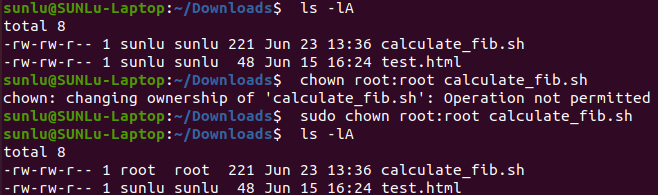
\includegraphics[width=350pt]{chapters/part-1/figures/chownexp.png}
	\caption{Change ownership and group of a file.} \label{ch:fm:fig:chownexp}
\end{figure}

\subsection{Change Permissions of a File or Directory}

Both the owner and the users with administrative privilege can change the ACL of a file or directory using \verb|chmod| as follows. The ACL, in this context, is called the mode of the item.
\begin{lstlisting}
$ chmod [<option>] <new_mode> <path>
\end{lstlisting}
For example, in Fig. \ref{ch:fm:fig:chmodexp}, \verb|g-w| is used to subtract ``writing'' permission from ``group'', and \verb|go+w| is used to add ``writing'' permission to `group'' and ``other'', respectively. Here, \verb|u|, \verb|g| and \verb|o| represents ``user'' (owner), ``group'' and ``other'', and \verb|r|, \verb|w| and \verb|x|, ``read'', ``write'' and ``execute'', respectively.
\begin{figure}[htbp]
	\centering
	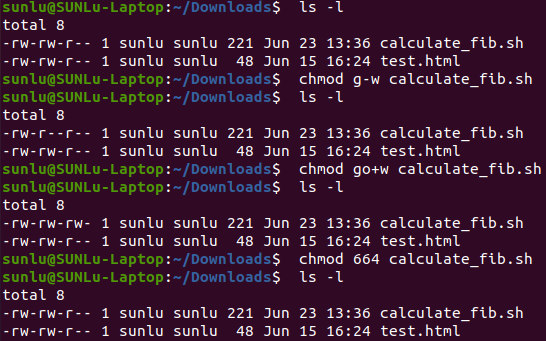
\includegraphics[width=350pt]{chapters/part-1/figures/chmodexp.png}
	\caption{Change 9-bit permission (mode) of a file.} \label{ch:fm:fig:chmodexp}
\end{figure}
Alternatively, 3-digit numbers such as \verb|664| as shown in Fig. \ref{ch:fm:fig:chmodexp} can also represent a permission. The first digit is associated with the permission given to the ``user'', where in this example \verb|6| (\verb|110B|) represents \verb|rw-|. Each ``1'' in the binary number is associated with a permission. The second and third digits are associated with the permission given to ``group'' and ``other'' respectively. Hence, \verb|664| would assign \verb|rw-rw-r--| to the file.

\subsection{Change Default Permissions}

The default ACL for a newly created file or directory is defined by \verb|umask|. Check its value by
\begin{lstlisting}
$ umask
\end{lstlisting}
And change its value temporarily in the opening shell by
\begin{lstlisting}
$ umask <new value>
\end{lstlisting}

The value of \verb|umask|, after converting to binary, represents the bits in the 9-bit permission system that is disabled. For example, a \verb|umask| value of \verb|002| represents \verb|rwxrwxr-x| in the 9-bit permission system, because the binary form of \verb|002|, \verb|000000010|, blocks the $8$-th bit in the permission.

To permanently change the value of \verb|umask|, configure it in \verb|.bashrc| as introduced in Section \ref{ch:sb:subsec:customizeshell}.

\section{Search through the System}

The most frequently used 3 searching actions are as follows.
\begin{itemize}
  \item Look for the location of a command using its name
  \item Look for the location of a file using its name (and other metadata such as size, permission, etc.)
  \item Look for the location of a file using a portion its content
\end{itemize}

Many approaches can be used to achieve the goals, some of which are introduced as follows.

\subsection{Look for a Command}

Use \verb|type| to look for a command as follows.
\begin{lstlisting}
$ type <command>
\end{lstlisting}

For example
\begin{lstlisting}
$ type cd
cd is a shell builtin
$ type python
python is /usr/bin/python
$ type ls
ls is aliased to `ls --color=auto'
\end{lstlisting}

\subsection{Looking for Files by Metadata}

Many Linux distributions come with built-in command \verb|locate| that can be used to quickly locate a file by (a fraction of) its path as follows. Notice that as long as a file or directory's full path contains the searched content, there is a chance that it will appear in the result. As a result, if the name of a directory is used for searching, all the items in that directory will likely to appear in the result (as their full paths contain the name of the directory).
\begin{lstlisting}
$ locate <file or path fraction>
\end{lstlisting}

The mechanism of \verb|locate| is explained as follows. The OS runs \verb|updatedb| in the background usually once a day to update an internal database that gathers the names of files, and \verb|locate| searches that database for the file. Notice that \verb|locate| may fail to find recently added files if it has not been added to the database by \verb|updatedb|. Besides, not all files' name are stored in that database by default, and a configuration file at \verb|/etc/updatedb.conf| determines which files' name to be included. It is also worth mentioning that it will take some time to run \verb|updatedb| for the first time, as it has a lot of things to add to the database during its initial run.

One may get confused by commands \verb|locate| and \verb|mlocate|. The two commands are very similar and they differ only beyond basic usage. Sometimes \verb|locate| is aliased to \verb|mlocate| when both functions are installed. In the scope of our discussion, we do not distinguish \verb|locate| and \verb|mlocate|.

An example of using \verb|locate|/\verb|mlocate| is given in Fig. \ref{ch:fm:fig:locateexp}. It can be seen from this example that the searching is done globally and does not rely on the current working directory.
\begin{figure}[htbp]
	\centering
	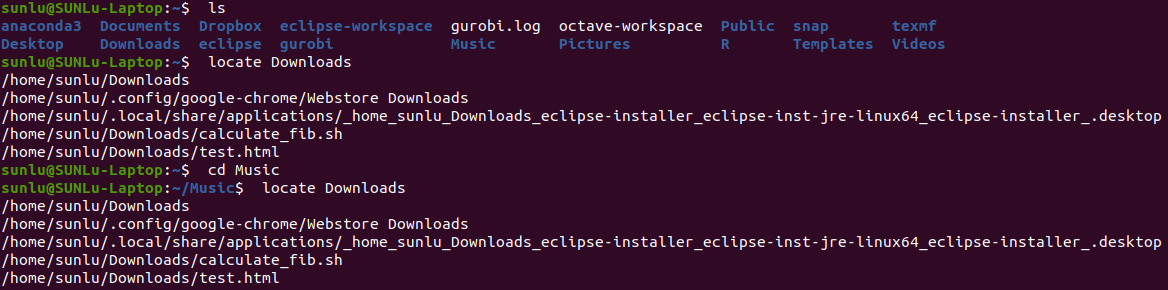
\includegraphics[width=350pt]{chapters/part-1/figures/locateexp.png}
	\caption{Search for files and directories using \textit{locate}.} \label{ch:fm:fig:locateexp}
\end{figure}

\subsection{Looking for Files by Variety of Properties}

It is worth mentioning that for safety and privacy reasons, \verb|mlocate| only shows the items that the user would be able to detect manually using \verb|cd| and \verb|ls| in the first place. Therefore, a regular user cannot locate any file under \verb|/root| our other users' home directory using this method.

A more common and widely accepted way of looking for a file by its variety of attributes is using \verb|find| as follows.
\begin{lstlisting}
$ find [<options>] [<path>] <expression>
\end{lstlisting}

The \verb|<options>| argument can be used to configure how the symbolic links should be handled. Symbolic links are like shortcut in Windows PC. It is a link that points to other directories of files. If \verb|-P| (default option) is used, the symbolic links are treated as the links themselves, but not the files they are linking to, whereas \verb|-L| does the opposite. Debugging modes and query optimization can also be enabled from \verb|<options>|. The \verb|<path>| argument specifies the directory from where the query is conducted. The \verb|<expression>| argument specifies the keyword and the query method.

The following are examples of using \verb|find| in different scenarios. The examples are taken from RedHat at \cite{redhat2022find}.

\vspace{0.1in}
\noindent \textbf{List everything in a directory and its subdirectories}
\vspace{0.1in}

\begin{lstlisting}
$ find ~/Documents -ls
3554235 0 drwxr-xr-x [...] 05:36 /home/seth/Documents/
3554224 0 -rw-rw-r-- [...] 05:36 /home/seth/Documents/Foo
3766411 0 -rw-rw-r-- [...] 05:36 /home/seth/Documents/Foo/foo.txt
\end{lstlisting}

\vspace{0.1in}
\noindent \textbf{Find files by name}
\vspace{0.1in}

Case sensitive: \verb|-name|
\begin{lstlisting}
$ find / -name "*Foo*txt" 2>/dev/null
/home/seth/Documents/Foo.txt
\end{lstlisting}

Case insensitive: \verb|-iname|
\begin{lstlisting}
$ find / -iname "*Foo*txt" 2>/dev/null
/home/seth/Documents/Foo.txt
/home/seth/Documents/foo.txt
/home/seth/Documents/foobar.txt
\end{lstlisting}

Wildcards such as \verb|*| can be used. Commonly used wildcards are given in Table \ref{ch:fm:tab:metacharacters}.

\vspace{0.1in}
\noindent \textbf{Find files by the content}
\vspace{0.1in}

\begin{lstlisting}
$ find ~/Documents/ -name "*txt" -exec grep -Hi penguin {} \;
/home/seth/Documents/Foo.txt:I like penguins.
/home/seth/Documents/foo.txt:Penguins are fun.
\end{lstlisting}
where in this example, \verb|-exec| allows executing a command to the findings. Notice that \verb|grep| by itself can also be used to search files by contents.

\vspace{0.1in}
\noindent \textbf{Find files by type}
\vspace{0.1in}

To find all files,
\begin{lstlisting}
$ find ~ -type f
/home/seth/.bash_logout
/home/seth/.bash_profile
/home/seth/.bashrc
/home/seth/.emacs
/home/seth/.local/share/keyrings/login.keyring
/home/seth/.local/share/keyrings/user.keystore
/home/seth/.local/share/gnome-shell/gnome-overrides-migrated
\end{lstlisting}
Specifically, to find empty files,
\begin{lstlisting}
$ find ~ -type f -empty
random.idea.txt
\end{lstlisting}

To find all subdirectories,
\begin{lstlisting}
$ find ~/Public -type d
find ~/Public/ -type d
/home/seth/Public/
/home/seth/Public/example.com
/home/seth/Public/example.com/www
/home/seth/Public/example.com/www/img
/home/seth/Public/example.com/www/font
/home/seth/Public/example.com/www/style
\end{lstlisting}

Use \verb|-maxdepth| to set the searching depth as follows.
\begin{lstlisting}
$ find ~/Public/ -maxdepth 1 -type d
/home/seth/Public/
/home/seth/Public/example.com
\end{lstlisting}

\vspace{0.1in}
\noindent \textbf{Find files by the timestamp it was accessed / changed / metadata changed}
\vspace{0.1in}

To find files whose latest modified time is at least 30 days ago (30 days ago or earlier), use
\begin{lstlisting}
 find /var/log -mtime +30
\end{lstlisting}
where \verb|-atime|, \verb|-ctime| and \verb|-mtime| search based on the number of days since each file was accessed, changed or had its metadata changed respectively. The alternatives \verb|-amin|, \verb|-cmin| and \verb|-mmin| work similarly in minutes. The \verb|+| indicates ``at least'' whereas \verb|-| indicates ``not more than''.

\section{File Archive}

The \verb|tar|, \verb|gzip| and \verb|zip| commands can all be used in files archive, but with different features, as given in Table \ref{ch:fm:tab:filearchivetools}.

\begin{table}
	\centering \caption{Commonly used file archive tools.}\label{ch:fm:tab:filearchivetools}
	\begin{tabularx}{\textwidth}{lX}
		\hline
		Directory & Description \\ \hline
		\verb|tar| & Save many files together into a single tape or disk archive, and can
		restore individual files from the archive. By default, it does not compress the files. However, \verb|-z| option can be used in combination of the command to add compression feature. \\ 
		\verb|gzip| & Compress or restore files. \\ 
		\verb|zip| & Compress multiple files one-by-one and integrate them together into a single file. \\
		\hline
	\end{tabularx}
\end{table}

Only \verb|tar| command is introduced here, as it is the most commonly used one among the three, and it can satisfy most use cases. A common way of using \verb|tar| is as follows. Use
\begin{lstlisting}
$ tar -cvzf <archive-file> <file1> <file2> <file3> ...
\end{lstlisting}
to archive and zip files, and
\begin{lstlisting}
$ tar -xvzf <archive-file>
\end{lstlisting}
to restore files from the archive file. The commonly used archive file name, in this scenario, is \verb|<filename>.tgz|.

The detailed explanation to all available options for \verb|tar| can be found using \verb|tar --help|. The most commonly used options are \verb|-c|, \verb|-x|, \verb|-z|, \verb|-f| and \verb|-v|, standing for creating compress tape, extracting (restoring) file, adding compressing feature, using file archive, and listing processed files in the console, respectively.















